\documentclass[12pt]{article}

\usepackage[english]{babel}
\usepackage[utf8]{inputenc}
\usepackage{sansmathfonts}
\usepackage[T1]{fontenc}
\renewcommand*\familydefault{\sfdefault} %% Only if the base font of the document is to be sans serif
\usepackage{multicol,lipsum}
\usepackage{amsmath,cancel}
\usepackage{amssymb,amsthm,dsfont,mathrsfs}
\usepackage[colorinlistoftodos]{todonotes}
\usepackage{geometry}
\geometry{
a4paper,
total={170mm,257mm},
left=20mm,
top=15mm,
bottom=22mm,
}
\usepackage{natbib}
\usepackage{soul}
\usepackage{setspace}
\usepackage{hyperref}
\usepackage{xcolor}
\usepackage{graphicx}
\usepackage{tikz}
\usepackage{siunitx}
\graphicspath{ {imagens/} }
\usepackage{fancyhdr}
\pagestyle{fancy}
\renewcommand{\headrulewidth}{0pt}

\color{darkgray}
\newcommand{\T}[1]{\vspace{0.4cm}\textbf{\large#1}}
\newcommand{\TW}[1]{\textbf{\large#1}}

\newcommand{\TM}[1]{\vspace{0.2cm} \textbf{#1}}

\newcommand{\M}[1]{
\vspace{-0.6cm}
\begin{flalign*}
#1&
\end{flalign*}
\vspace{-0.6cm}
}


\definecolor{bluebell}{rgb}{0.25, 0.35, 0.89} 
\definecolor{laranja}{rgb}{0.87, 0.48, 0.25} 
\definecolor{verde}{rgb}{0, 0.54, 0.44} 
\definecolor{babypink}{rgb}{1, 0.42, 0.52} 
\definecolor{rosa}{rgb}{1, 0.72, 0.77} 
\definecolor{cinza}{rgb}{0.3, 0.3, 0.3}  
\definecolor{iris}{rgb}{0.25, 0.35, 0.89}  
\definecolor{babyblue}{rgb}{0.13, 0.59, 0.95}

\setlength\columnsep{30pt}

\setlength{\parindent}{0cm}
\setlength{\fboxrule}{1.3pt}  % <-- Aumenta a espessura

\newcommand{\Formula}[1]{
\begin{center}
\color{iris}
\fcolorbox{rosa}{white}{
\(
\begin{array}{c}
#1
\end{array}
\)
}
\color{cinza}
\end{center}
}

\begin{document}
\pagenumbering{gobble}
\setstretch{1.3}


\includegraphics[width=4cm]{Logo2.png}
\begin{center}
    \textbf{\Huge \textcolor{bluebell}{Função Exponencial}}
\end{center}

\begin{multicols}{2}

% ── DEFINIÇÃO ──────────────────────────────────────────────────────────────
\TW{Definição}

A função exponencial é definida por $f(x) = a^x$, onde a \textbf{base} $a$ é uma constante
real positiva diferente de 1 ($a > 0$ e $a \neq 1$) e o \textbf{expoente} $x$ é a variável
independente.

\Formula{f(x) = a^x,\quad a > 0,\; a \neq 1}

O \textbf{domínio} é $\mathbb{R}$ e a \textbf{imagem} é $(0,+\infty)$ — a função nunca
é zero nem negativa. A restrição $a \neq 1$ evita a função constante $1^x = 1$.

\TM{Exemplos:}

\textbf{Base 2 (crescente):} $f(x) = 2^x$

$f(3) = 2^3 = 8$ \hfill $f(-2) = 2^{-2} = \tfrac{1}{4}$ \hfill $f(0) = \boxed{1}$

\textbf{Base $\tfrac{1}{2}$ (decrescente):} $f(x) = \left(\tfrac{1}{2}\right)^x$

$f(3) = \tfrac{1}{8}$ \qquad $f(-2) = 4$ \qquad Nota: $\left(\tfrac{1}{2}\right)^x = 2^{-x}$

\fcolorbox{laranja}{white}{\parbox{0.85\linewidth}{
\small\textbf{Propriedade:} $a^0 = 1$ para qualquer base válida. O gráfico de toda função
exponencial passa pelo ponto $(0, 1)$.
}}

% ── GRÁFICO ────────────────────────────────────────────────────────────────
\TW{Gráfico}

\begin{center}
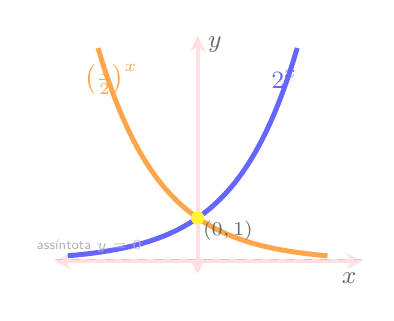
\begin{tikzpicture}[scale=0.55]
\tikzstyle{eixo}=[pink!50!white, line width=1.5pt]
\draw[eixo, stealth-stealth] (-3.3,0) -- (3.8,0);
\draw[eixo, stealth-stealth] (0,-0.3) -- (0,5.2);
\draw[blue!60!white, line width=1.8pt, domain=-3:2.3, samples=60]
    plot (\x, {exp(\x * 0.6931)});
\draw[orange!70!white, line width=1.8pt, domain=-2.3:3, samples=60]
    plot (\x, {exp(-\x * 0.6931)});
\filldraw[yellow!80!white] (0,1) circle (4pt);
\node[black!60!white] at (3.5,-0.4) {\small$x$};
\node[black!60!white] at (0.4,5.0) {\small$y$};
\node[black!60!white] at (0.7,0.7) {\scriptsize$(0,1)$};
\node[blue!60!white]   at (2.0,4.2) {\small$2^x$};
\node[orange!70!white] at (-2.0,4.2) {\small$\left(\tfrac{1}{2}\right)^x$};
\draw[dashed, gray!40!white] (-3.3,0.03) -- (3.8,0.03);
\node[gray!60!white] at (-2.5,0.35) {\tiny assíntota $y=0$};
\end{tikzpicture}
\end{center}

$a > 1$: função \textbf{crescente}; quando $x \to -\infty$, $f(x) \to 0^+$.

$0 < a < 1$: função \textbf{decrescente}; quando $x \to +\infty$, $f(x) \to 0^+$.

% ── NÚMERO DE EULER ────────────────────────────────────────────────────────
\TW{Número de Euler}

O número $\mathrm{e}$ é a base da \textbf{exponencial natural}:

\Formula{\mathrm{e} = \lim_{n \to \infty}\!\left(1 + \dfrac{1}{n}\right)^n \approx 2{,}71828\ldots}

$e^1 \approx 2{,}718$ \quad $e^2 \approx 7{,}389$ \quad $e^0 = 1$ \quad $\ln(\mathrm{e}) = 1$

A derivada de $e^x$ é ela mesma — propriedade única que a torna fundamental em cálculo,
física e probabilidade.

% ── EQUAÇÕES EXPONENCIAIS ──────────────────────────────────────────────────
\TW{Equações Exponenciais}

A incógnita está no expoente. Estratégia: \textbf{igualar as bases} ou aplicar
\textbf{logaritmo}.

\TM{Tipo 1 — igualação de bases:}

$2^x = 32 \;\Rightarrow\; 2^x = 2^5 \;\Rightarrow\; \boxed{x = 5}$

$3^{2x-1} = 27 \;\Rightarrow\; 3^{2x-1} = 3^3 \;\Rightarrow\; 2x = 4 \;\Rightarrow\; \boxed{x = 2}$

$4^x = 8 \;\Rightarrow\; 2^{2x} = 2^3 \;\Rightarrow\; 2x = 3 \;\Rightarrow\; \boxed{x = \tfrac{3}{2}}$

$9^x = \dfrac{1}{27} \;\Rightarrow\; 3^{2x} = 3^{-3} \;\Rightarrow\; \boxed{x = -\tfrac{3}{2}}$

\TM{Tipo 2 — bases diferentes (logaritmo):}

$2^x = 5$; aplica $\log$: $x \cdot \log 2 = \log 5$

\M{x &= \dfrac{\log 5}{\log 2} \approx \dfrac{0{,}699}{0{,}301} \approx 2{,}32}

\TM{Tipo 3 — equação quadrática (substituição):}

$4^x - 5 \cdot 2^x + 4 = 0$; seja $y = 2^x$:

$y^2 - 5y + 4 = 0 \;\Rightarrow\; (y-1)(y-4) = 0$

$y = 1 \Rightarrow x = 0$ \quad e \quad $y = 4 \Rightarrow x = 2$

% ── APLICAÇÕES ─────────────────────────────────────────────────────────────
\TW{Aplicações}

\TM{Crescimento — bactérias:}

Colônia dobra a cada hora; 500 iniciais. Após 6 horas:

$N(t) = 500 \cdot 2^t \;\Rightarrow\; N(6) = 500 \cdot 64 = \boxed{32\,000}$ bactérias

\TM{Decaimento — Carbono-14:}

Meia-vida 5730 anos; 200 g iniciais. Após 11460 anos (2 meias-vidas):

\M{M &= 200 \cdot \left(\tfrac{1}{2}\right)^{\!2} = \boxed{50}\text{ g}}

\TM{Juros compostos:}

\Formula{M = C \cdot (1 + i)^t}

R\$\,2000 a 5\%/mês por 4 meses: $(1{,}05)^4 \approx 1{,}2155$

$M \approx$ R\$\,2431,01 (vs.\ R\$\,2400 nos juros simples — a diferença é o rendimento
sobre os juros acumulados)

\end{multicols}

\lfoot{\scriptsize © Copyright, Pratique Já}
\cfoot{\large \textcolor{bluebell}{pratiqueja.com}}
\end{document}
